\documentclass[a4paper,14pt]{extreport}
\usepackage[utf8]{inputenc}
\usepackage[T2A]{fontenc}
\usepackage[russian]{babel}
\usepackage{eufrak}
% поля:
\usepackage[left=2.5cm, right=2cm, top=2cm, bottom=2cm]{geometry}
\linespread{1}
\usepackage{indentfirst} % отделять первую строку раздела абзацным отступом
\setlength\parindent{5ex}
\addto{\captionsrussian}{\renewcommand*{\contentsname}{Содержание}}
\usepackage[hidelinks]{hyperref} % гиперссылки в содержании
\usepackage{graphicx}
\usepackage{float}
\usepackage{amsmath}
\renewcommand*{\thesection}{\arabic{section}}

\begin{document}
	
\begin{titlepage}
	\begin{center}
		\large
		МИНИСТЕРСТВО ОБРАЗОВАНИЯ И НАУКИ\\ РОССИЙСКОЙ ФЕДЕРАЦИИ
		
		\textbf{Федеральное агентство по образованию}
		\vspace{0.5cm}
		
		УНИВЕРСИТЕТ ИТМО
		\vspace{0.25cm}
		
		Факультет компьютерных технологий и управления
		
		Кафедра систем управления и информатики
		\vfill
		
		
		Студент: Артемов Кирилл\\
		группа P4135\\
		
		\textsc{Лабораторная работа №3}\\[5mm]
		
		{\LARGE Планирование траектории движения с использованием сплайнов}
		\bigskip
		
	\end{center}
	\vfill
	
	\newlength{\ML}
	\settowidth{\ML}{«\underline{\hspace{0.7cm}}» \underline{\hspace{2cm}}}
	\hfill\begin{minipage}{0.4\textwidth}
		Преподаватель\\
		\underline{\hspace{\ML}} А.\,А.~Пыркин\\
		«\underline{\hspace{0.7cm}}» \underline{\hspace{2cm}} 2016 г.
	\end{minipage}%
	\bigskip
	
	\vfill
	
	\begin{center}
		Санкт-Петербург, 2016 г.
	\end{center}
\end{titlepage}

\pagenumbering{gobble}
\section{Цель работы}
Решить задачу планирования траектории движения манипулятора методом сплайнов.

\section{Исходные данные}
	Заданы четыре точки в пространстве, через которые должен пройти схват манипулятора. А также его скорости и ускорения в начальных точках. 
	\begin{center}
		$I = (x^I, y^I, z^I)$\\
		$D = (x^D, y^D, z^D)$\\
		$A = (x^A, y^A, z^A)$\\
		$F = (x^F, y^F, z^F)$\\
	\end{center}

	\begin{figure}[H]
	\center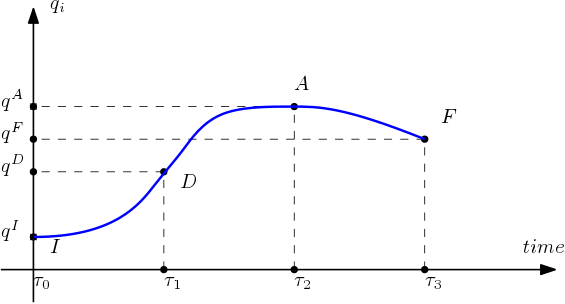
\includegraphics[width=0.8\linewidth]{trajectory.png}
	\caption{Траектория. Зависимость вектора обобщенных координат q от времени}
	\label{fig:scr1}
	\end{figure}

\section{Ход выполнения работы}
	Прежде чем приступить к планированию траектории движения, необходимо опредилить конфигурацию манипулятора в четырех заданных точках. Для этого, для каждой из точек, решается обратная задача кинемматики, в результате чего получается четыре вектора обобщенных координат $q^I, q^D, q^A, q^F$.
	
	Далее, необходимо выбрать способ разбиения траектории на участки. В этой лабораторной работе им стал способ разбиение траектории на полиномы степеней 4-3-4.
	
	Таким образом, траектория изменения каждой из обобщенных координат разбивается на три участка. Превый участок, задающий движение между начальной точкой $I$ и точко ухода $D$, описывается полиномом четвертой степени. Второй участок траектории между точкой ухода $D$ и точкой подхода $A$ описывается полиномом третьей степени. Последний участок между точками подхода $A$ и конечной $F$ описывается полиномом четвертой степени.
	
	\subsection{Расчет 4-3-4 траектории}
	В связи с тем, что для каждого участка траектории требуется определить N траекторий обобщенных координат, удобно воспользоваться нормированным временем $t \in [0, 1]$. Это позволяет достичь единообразия уравнений, описывающих изменение каждой из обобщенных координат на каждом уччастке траектории.
	\begin{center}
		$t = \frac{\tau - \tau_{i-1}}{\tau_{i} - \tau_{i-1}};$
		$\tau \in [\tau_{i-1}, \tau_{i}]; t \in [0, 1]$	
			\\
	\end{center}
	 
	Траектория движения $i$ обобщенной координаты задется в виде последовательности полиномов. Полиномы выражены в нормированном времени. Скорости и ускорения находят взятием соответствующей производной от представленной ниже системы.
	\begin{equation*}
	q_i(t) = 
	\begin{cases}
		a_0 + a_1  t + a_2  t^2 + a_3 t^3 + a_4 t^4 \\
		b_0 + b_1  t + b_2  t^2 + b_3 t^3  \\
		c_0 + c_1  t + c_2  t^2 + c_3 t^3 + c_4 t^4
	\end{cases}
	\end{equation*}
	 
	 Граничные условия, которым должна удовлетворять система полиномов представлены в таблице 1. 
		\begin{table}[H]
		\caption{\label{tab:canonsummary}Граничные условия}
		\begin{center}
			\begin{tabular}{|c|c|c|}
				\hline
				Первый участок & Второй участок & Последний участок \\
				\hline
				$q_{1i}(0)= q^I_i$ 		& $q_{2i}(0)= q^D_i$					& $q_{ni}(0)= q^A_i$\\
				$\dot q_{1i}(0) = v^I$	& $\dot q_{2i}(0) = \dot q_{1i}(1)$ 	& $\dot q_{ni}(0) = \dot q_{2i}(1)$\\
				$\ddot q_{1i}(0) = a^I$	& $\ddot q_{2i}(0) = \ddot q_{1i}(1)$	& $\ddot q_{ni}(0) = \ddot q_{2i}(1)$\\
				$q_{1i}(1) = q^D_i$		& $q_{2i}(1) = q^A_i$				&$q_{ni}(1) = q^F_i$\\
				&& $q_{ni}(1) = v^F$\\
				&& $q_{ni}(1) = a^F$\\
				\hline
			\end{tabular}
		\end{center}
	\end{table} 
	
	Применим граничные условия и нормированное время для того, чтобы склеить полиномы меду собой в заданных точках.
	
	\begin{enumerate}
		\item $t = 0$
	\begin{equation*}
		q_i(0) = 
		\begin{cases}
		a_0 = q^I \\
		b_0 = q^D \\
		c_0 = q^A
		\end{cases}
	\end{equation*}		
	\begin{equation*}
		\dot q_i(0) = 
		\begin{cases}
		a_1 = v^I \\
		b_1 = \dot q_1(1) \\
		c_1 = \dot q_2(1)
		\end{cases}
	\end{equation*}	
	\begin{equation*}
		\ddot q_i(0) = 
		\begin{cases}
		2 a_2 = a^I \\
		2 b_2 = \ddot q_1(1)\\
		2 c_2 = \ddot q_2(1)
		\end{cases}
	\end{equation*}	

		\item $t = 1$
	\begin{equation*}
		q_i(1) = 
		\begin{cases}
		a_0 + a_1 + a_2 + a_3  + a_4 = q^D\\
		b_0 + b_1 + b_2 + b_3 = q^A \\
		c_0 + c_1 + c_2  + c_3 + c_4 = q^F 
		\end{cases}
	\end{equation*}	
	\begin{equation*}
		\dot q_i(1) = 
		\begin{cases}
		a_1 + 2 a_2 + 3 a_3  + 4 a_4 = v^D\\
		b_1 + 2 b_2 + 3 b_3 = v^A \\
		c_1 + 2 c_2 + 3 c_3 + 4 c_4 = v^F 
		\end{cases}
	\end{equation*}	
	\begin{equation*}
		\ddot q_i(1) = 
		\begin{cases}
		2 a_2 + 6 a_3  + 12 a_4 = a^D\\
		2 b_2 + 6 b_3 = a^A \\
		2 c_2 + 6 c_3 + 12 c_4 = a^F 
		\end{cases}
	\end{equation*}	
	\end{enumerate}
	Далее, запишем четырнадцать уравнений, необходимых для решения уравнения движения. Принимая $v^I = 0, a^I = 0$, получим:
	\begin{align*}
		q^I &= a_0\\
		0 &= a_1\\
		0 &= a_2\\
		q^D - q^I &= a_3 + a_4\\
		q_D &= b_0\\
		0 &= b_1 - 3 a_3 - 4 a_4\\
		0 &= b_2 - 3 a_3 - 6 a_4\\
		q^A - q^D &= b_1 + b_2 + b_3\\
		q^A &= c_0\\
		0 &= c_1 - b_1 - 2 b_2 -3 b_3\\
		0 &= c_2 - b_2 - 3 b_3\\
		q^F - q^A &= c_1 + c_2 + c_3 + c_4 \\
		0 &= c_1 + 2 c_2 + 3 c_3 + 4 c_4\\
		0 &= 2 c_2 + 6 c_3 + 12 c_4
	\end{align*}
	
	Теперь, из того, что стоит слева от знака равенства составляем вектор-столбец $b$ известных величин, а из того, что справа -- матрицу коэффициентов $C$. Составляем матричное уравнение:
	
	\begin{equation}
		Cx = b
	\end{equation}
	
	И наконец, задаем время движения манипулятора между точками и вычисляем для заданных интервалов времени значения полиномов. Решая прямую задачу кинематики находим декартовы координаты схвата в каждый из заданных моментов времени.
	
	\begin{figure}[H]
	 	\center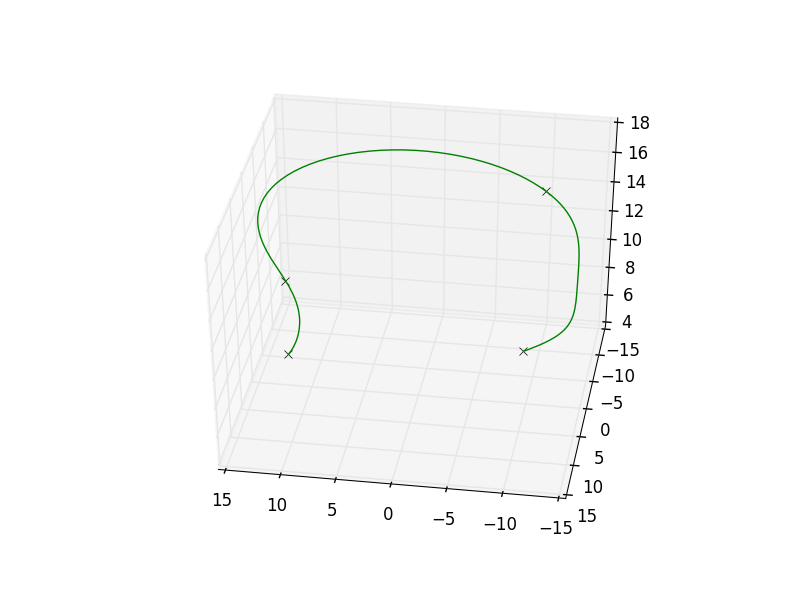
\includegraphics[width=1\linewidth]{trajectory2.png}
	 	\caption{Траектория движения схвата манипулятора}
	 	\label{fig:scr1}
	\end{figure}

	\section{Вывод}
	Мною была решена задача планирования траектории движения схвата манипулятора с использованием метода сплайнов. Как видно из рисунка 2, траектория удовлетворяет предъявляемым к ней требованиям, а именно: проходит через заданные точки, при этом без скачков, что соответствует поставленной задаче.

\end{document}


